\section{Complexity of current standards and protocols}
\label{sec:complexity_of_current_standards_and_protocols}
QUIC integration with TLS as well as stream multiplexing and combination of reliable and unreliable messages can significantly reduce complexity of current systems and standards.
This section outlines how QUIC can be used in SSH protocol and WebRTC standard.
\subsection{WebRTC}
WebRTC is a standard that enables peer to peer (P2P) multimedia connections in web browsers when both peers are behind NATs without using any plugins.
This standard is natively implemented by all major browsers.
WebRTC is called protocol umbrella which means it combines a lot of different separate protocols to make things work.
In WebRTC there are two planes -- media plane and signaling plane.
The former is responsible for relaying both media data (audio, video) and non-media data (chat messages, uploading and downloading files, etc.).
The later is responsible for negotiating session parameters like audio and video codecs or transport addresses.
This architecture is presented in figure \ref{fig:webrtc-stack}

\begin{figure}[h]
    \centering
    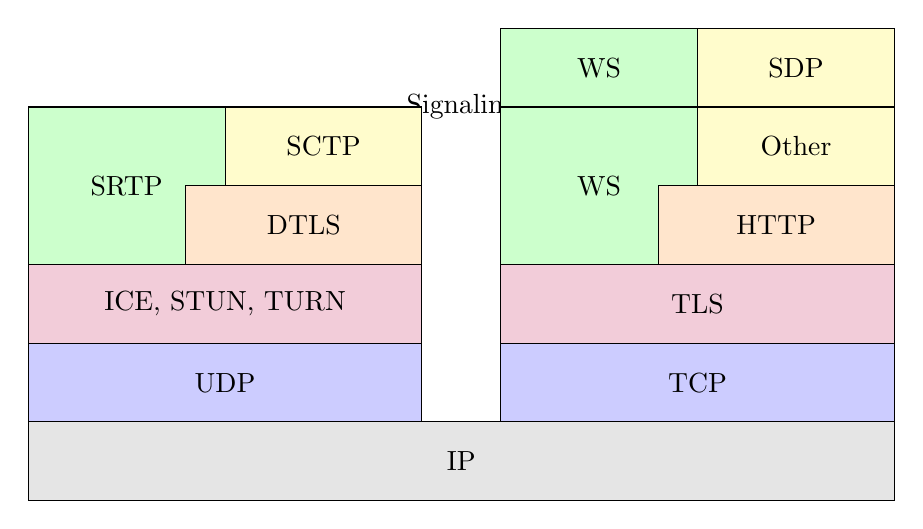
\begin{tikzpicture}
        % signaling plane
        \node at (6,5) {Signaling Plane};
        \filldraw [fill=green!20] (6, 5) rectangle node{WS} (8.5, 6); \filldraw [fill=yellow!20] (8.5, 5) rectangle node{SDP} (11, 6);
        \filldraw [fill=green!20] (6, 3) rectangle node{WS} (8.5, 5); \filldraw [fill=yellow!20] (8.5, 4) rectangle node{Other} (11, 5);
        \filldraw [fill=orange!20] (8, 3) rectangle node{HTTP} (11, 4);
        \filldraw [fill=purple!20] (6, 2) rectangle node{TLS} (11, 3);
        \filldraw [fill=blue!20] (6, 1) rectangle node{TCP} (11, 2);
        
        % media plane
        \filldraw [fill=green!20] (0, 3) rectangle node{SRTP} (2.5, 5); \filldraw [fill=yellow!20] (2.5, 4) rectangle node{SCTP} (5, 5);
        \filldraw [fill=orange!20] (2, 3) rectangle node{DTLS} (5, 4);
        \filldraw [fill=purple!20] (0, 2) rectangle node{ICE, STUN, TURN} (5, 3);
        \filldraw [fill=blue!20] (0, 1) rectangle node{UDP} (5, 2);
        
        % ip
        \filldraw [fill=gray!20] (0, 0) rectangle node{IP} (11, 1);
    \end{tikzpicture}
    \caption{WebRTC stack.}
    \label{fig:webrtc-stack}
\end{figure}

\subsubsection{Media plane}
In media plane, media data are carried using SRTP protocol which stands for Secure Real Time Protocol.
SRTP is encrypted version of RTP protocol and provides packets with some additional information that is not present in headers of UDP datagrams.
This information includes timestamps -- to know how fast data should be passed to video or audio decoder, sequence numbers -- to perform reordering, payload type -- to know which codec is used.
On the other hand, non-media data is carried by SCTP.
SRTP protocol uses cryptografic context negotiated during DTLS handshake for encrypting RTP packets payload.
SCTP is encapsulated in DTLS datagrams.
Below SRTP and SCTP there are ICE, STUN and TURN.
They are used for establishing a connection between peers even when both of them are behind NATs.
At the end, in most cases everything is carried in UDP datagrams.
However, in some specific scenarios (e.g. when some network blocks UDP traffic or allows only for traffic on port 443) TCP may be used.

\subsubsection{Signaling plane}

Main protocol used in signaling plane is Session Description Protocol (SDP).
It defines format of messages that carry information about number of media tracks, their codecs, relationship between them, etc.
WebRTC does not define how to exchange these messages between peers.
Instead, user (i.e. someone using WebRTC API) is responsible for conveying SDP messages.
This in a lot of cases is done using separate connection over WebSockets (WS).
Whole WebRTC infrastructure is presented in figure \ref{fig:webrtc-architecture}

% \begin{figure}[h]
%     \centering
%     % media plane
%     \begin{tikzpicture}
%         \draw (0, 0) node (pc_a)  {
\includegraphics{cisco_icons/pc.eps}};
%         \draw (10, 0) node (pc_b) {
\includegraphics{cisco_icons/pc.eps}};
%         \draw (5, 2) node (signaling_server) {
\includegraphics{cisco_icons/workstation.eps}}
%         \draw [<->, postaction={decorate,decoration={raise=2ex, text along path,text align=center,text={audio/video/non-media data}}}] (pc_a) -- (pc_b);
%         \draw [<->, postaction={decorate,decoration={raise=2ex, text along path,text align=center,text={signaling messages}}}] (pc_a.north) to [bend left=45] (pc_b.north);
%     \end{tikzpicture}
%     \label{fig:webrtc-architecture}
%     \caption{WebRTC architecture}
% \end{figure}

% \begin{figure}[h]
%     \centering
%     \begin{subfigure}[b]{0.4\textwidth}
%     \begin{tikzpicture}
%         \filldraw [fill=green!20] (0, 3) rectangle node{SRTP} (2.5, 5); \filldraw [fill=yellow!20] (2.5, 4) rectangle node{SCTP} (5, 5);
%         \filldraw [fill=orange!20] (2, 3) rectangle node{DTLS} (5, 4);
%         \filldraw [fill=purple!20] (0, 2) rectangle node{ICE, STUN, TURN} (5, 3);
%         \filldraw [fill=blue!20] (0, 1) rectangle node{UDP} (5, 2);
%         \filldraw [fill=gray!20] (0, 0) rectangle node{IP} (5, 1);
%     \end{tikzpicture}
%     \caption{WebRTC stack.}
%     \label{fig:webrtc-stack}
%     \end{subfigure}
%     \hfill
%     \begin{subfigure}[b]{0.4\textwidth}
%     \begin{tikzpicture}
%         \filldraw [fill=green!20] (0, 4) rectangle node{SRTP} (5, 5);
%         \filldraw [fill=orange!20] (0, 3) rectangle node{QUIC} (5, 4);
%         \filldraw [fill=purple!20] (0, 2) rectangle node{ICE, STUN, TURN} (5, 3);
%         \filldraw [fill=blue!20] (0, 1) rectangle node{UDP} (5, 2);
%         \filldraw [fill=gray!20] (0, 0) rectangle node{IP} (5, 1);
%     \end{tikzpicture}
%     \caption{WebRTC stack with QUIC.}
%     \label{fig:quic-webrtc-stack-comparision}
%     \end{subfigure}
%     \caption{Comparison of current WebRTC stack and alternative WebRTC stack when using QUIC protocol.}
% \end{figure}

Thanks to QUIC we could probably get rid of dedicated congestion control (cc) protocol, SCTP and DTLS. 
There is also no need to use extension to RTP that provides encryption rules.
Instead we could use encryption mechanism provided with QUIC i.e. packets would be encrypted using TLS 1.3.

\subsection{SSH}
Secure Shell protocol allows for secure connections to remote machines over insecure network. 
It defines channels where each channel can be terminal session, forwarded connections etc. \cite{rfc4254}.
Channels are flow controlled.
One SSH connection can multiplex multiple SSH channels.
SSH uses TCP under the hood which is also flow controlled.
Figure \ref{fig:ssh-connection} presents architecture of SSH connection.

\begin{figure}[h]
  \begin{subfigure}[b]{0.4\textwidth}
    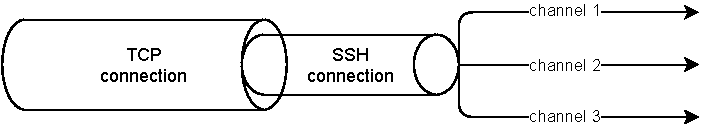
\includegraphics[width=\textwidth]{img/__06__current_standards_and_protocols/ssh.pdf}
    \caption{SSH connection architecture.}
    \label{fig:ssh-connection}
  \end{subfigure}
  \hfill
  \begin{subfigure}[b]{0.4\textwidth}
    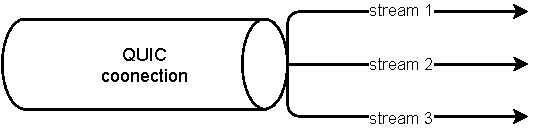
\includegraphics[width=\textwidth]{img/__06__current_standards_and_protocols/quic_ssh.pdf}
    \caption{Alternative SSH connection architecture with QUIC protocol.}
    \label{fig:quic-ssh-connection}
  \end{subfigure}
  \caption{Comparison of current SSH connection architecture and alternative SSH connection architecture using QUIC protocol.}
\end{figure}

According to \cite{bider-ssh-quic-09}, using QUIC connection we could remove one level of flow control, reduce connection handshakes from two (one for TCP and one for SSH) to one (only for QUIC) and use streams as SSH channels.
This approach is presented on figure \ref{fig:quic-ssh-connection}.
